\section{Date: 2026-08-15}
\noindent \textbf{Series ID: WFRBSTP1302} 

\noindent This series is titled Share of Other Loans And Advances (Assets) Held by the Top 0.1\% (99.9th to 100th Wealth Percentiles) and has a frequency of Quarterly. The units are Percent of Aggregate and the seasonal adjustment is Not Seasonally Adjusted.The observation start date is 1989-07-01 and the observation end date is 2026-01-01.The popularity of this series is 2. \\ 

\noindent \textbf{Series ID: CSESFT02CZM460S} 

\noindent This series is titled Consumer Opinion Surveys: Economic Situation: Future Tendency for Czechia and has a frequency of Monthly. The units are Percentage balance and the seasonal adjustment is Seasonally Adjusted.The observation start date is 1995-01-01 and the observation end date is 2026-06-01.The popularity of this series is 1. \\ 

\subsection{Raw Regression}
\noindent Regresses the two series against each other directly. A significant result here can come just as easily from both series sharing a long-run trend as from any real relationship.

\begin{center}
\begin{tabular}{lclc}
\toprule
\textbf{Dep. Variable:}           & value\_fred\_CSESFT02CZM460S & \textbf{  R-squared:         } &     0.019   \\
\textbf{Model:}                   &             OLS              & \textbf{  Adj. R-squared:    } &     0.011   \\
\textbf{Method:}                  &        Least Squares         & \textbf{  F-statistic:       } &     2.436   \\
\textbf{Date:}                    &       Sat, 15 Aug 2026       & \textbf{  Prob (F-statistic):} &    0.121    \\
\textbf{Time:}                    &           12:13:07           & \textbf{  Log-Likelihood:    } &   -520.13   \\
\textbf{No. Observations:}        &               125            & \textbf{  AIC:               } &     1044.   \\
\textbf{Df Residuals:}            &               123            & \textbf{  BIC:               } &     1050.   \\
\textbf{Df Model:}                &                 1            & \textbf{                     } &             \\
\textbf{Covariance Type:}         &          nonrobust           & \textbf{                     } &             \\
\bottomrule
\end{tabular}
\begin{tabular}{lcccccc}
                                  & \textbf{coef} & \textbf{std err} & \textbf{t} & \textbf{P$> |$t$|$} & \textbf{[0.025} & \textbf{0.975]}  \\
\midrule
\textbf{const}                    &     -17.3335  &        3.367     &    -5.148  &         0.000        &      -23.999    &      -10.668     \\
\textbf{value\_fred\_WFRBSTP1302} &       0.1411  &        0.090     &     1.561  &         0.121        &       -0.038    &        0.320     \\
\bottomrule
\end{tabular}
\begin{tabular}{lclc}
\textbf{Omnibus:}       &  5.838 & \textbf{  Durbin-Watson:     } &    0.334  \\
\textbf{Prob(Omnibus):} &  0.054 & \textbf{  Jarque-Bera (JB):  } &    5.818  \\
\textbf{Skew:}          & -0.489 & \textbf{  Prob(JB):          } &   0.0545  \\
\textbf{Kurtosis:}      &  2.599 & \textbf{  Cond. No.          } &     89.7  \\
\bottomrule
\end{tabular}
%\caption{OLS Regression Results}
\end{center}

Notes: \newline
 [1] Standard Errors assume that the covariance matrix of the errors is correctly specified.

\begin{figure}
\centering
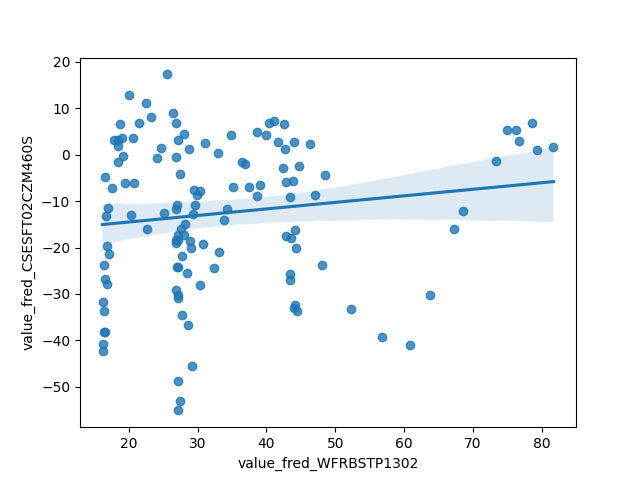
\includegraphics[scale = 0.9]{plots/plot_2026-08-15.png}
\caption{Raw Regression Plot for 2026-08-15}
\end{figure}
\newpage
\subsection{Detrended Regression}
\noindent Regresses the residuals of each series after removing its own linear time trend, so a shared trend can no longer drive the result on its own. A relationship that stays significant here is better evidence of a genuine link between the two series.

\begin{center}
\begin{tabular}{lclc}
\toprule
\textbf{Dep. Variable:}                      & value\_fred\_CSESFT02CZM460S\_detrended & \textbf{  R-squared:         } &     0.006   \\
\textbf{Model:}                              &                   OLS                   & \textbf{  Adj. R-squared:    } &    -0.002   \\
\textbf{Method:}                             &              Least Squares              & \textbf{  F-statistic:       } &    0.7443   \\
\textbf{Date:}                               &             Sat, 15 Aug 2026            & \textbf{  Prob (F-statistic):} &    0.390    \\
\textbf{Time:}                               &                 12:13:07                & \textbf{  Log-Likelihood:    } &   -520.09   \\
\textbf{No. Observations:}                   &                     125                 & \textbf{  AIC:               } &     1044.   \\
\textbf{Df Residuals:}                       &                     123                 & \textbf{  BIC:               } &     1050.   \\
\textbf{Df Model:}                           &                       1                 & \textbf{                     } &             \\
\textbf{Covariance Type:}                    &                nonrobust                & \textbf{                     } &             \\
\bottomrule
\end{tabular}
\begin{tabular}{lcccccc}
                                             & \textbf{coef} & \textbf{std err} & \textbf{t} & \textbf{P$> |$t$|$} & \textbf{[0.025} & \textbf{0.975]}  \\
\midrule
\textbf{const}                               &   -4.054e-13  &        1.399     &  -2.9e-13  &         1.000        &       -2.769    &        2.769     \\
\textbf{value\_fred\_WFRBSTP1302\_detrended} &       0.1123  &        0.130     &     0.863  &         0.390        &       -0.145    &        0.370     \\
\bottomrule
\end{tabular}
\begin{tabular}{lclc}
\textbf{Omnibus:}       &  5.827 & \textbf{  Durbin-Watson:     } &    0.334  \\
\textbf{Prob(Omnibus):} &  0.054 & \textbf{  Jarque-Bera (JB):  } &    5.696  \\
\textbf{Skew:}          & -0.475 & \textbf{  Prob(JB):          } &   0.0580  \\
\textbf{Kurtosis:}      &  2.564 & \textbf{  Cond. No.          } &     10.7  \\
\bottomrule
\end{tabular}
%\caption{OLS Regression Results}
\end{center}

Notes: \newline
 [1] Standard Errors assume that the covariance matrix of the errors is correctly specified.

\begin{figure}
\centering
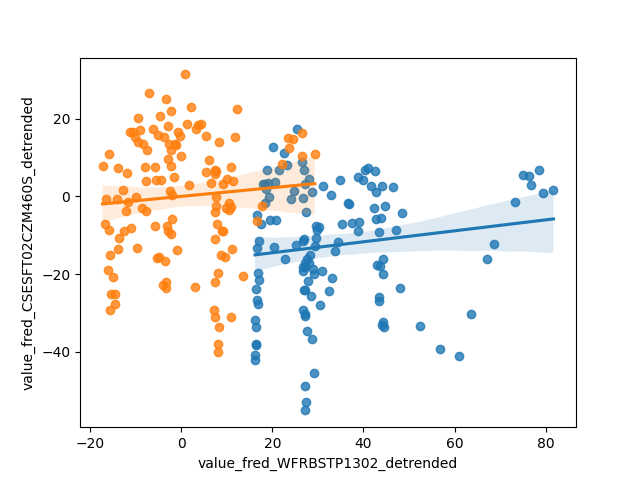
\includegraphics[scale = 0.9]{plots/plot_2026-08-15_detrended.png}
\caption{Detrended Regression Plot for 2026-08-15}
\end{figure}
\newpage
